%!TEX root =  main.tex
%!TEX encoding = UTF-8 Unicode
\chapter{推薦システムの実行過程}
\label{chap:oipmodel}

\begin{figure}
\centering
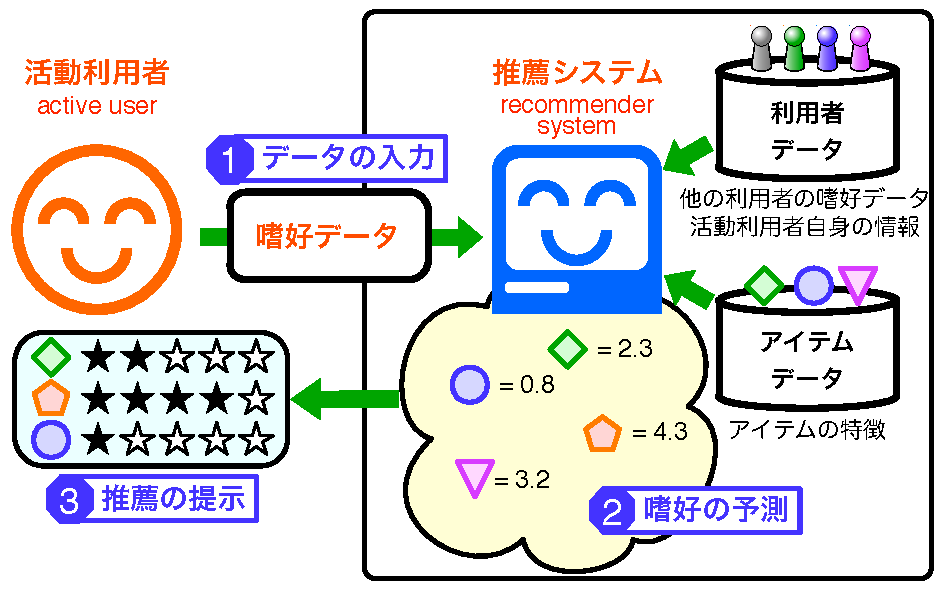
\includegraphics[width=0.8\fullwidth]{oipmodel.pdf}
\caption{推薦システムの実行過程(O-I-Pモデル)}
\label{fig:oipmodel}
\end{figure}

ここまでは,推薦システムを分類し,設計にあたって考慮すべき事項について述べてきた.ここでは,推薦システムがどのように実現されるかを見てゆこう.
推薦システムは,図\ref{fig:oipmodel}のように,データの入力,嗜好の予測,そして推薦の提示の三つの段階で推薦を行う.
これは\term{O-I-Pモデル}{output-input-process model}\cite{sigchi:03:01}とも呼ばれる.以下,これらの各段階の概要について述べる.

\begin{description}[style=nextline]
\item[データの入力]
推薦システムを利用して,推薦を受けようとしている人を\term{活動利用者}{active user}と呼ぶ.
活動利用者は自身の\termmain{嗜好データ}{preference data}を推薦システムに入力する.
嗜好データとは,いろいろなアイテムについての関心や好みの度合いを数値化したデータである.
この嗜好データの代わりに,関心のあるアイテムについてのより具体的な記述を検索質問や批評として,活動利用者に入力させるシステムもある.
また,推薦には,他の利用者の嗜好データ,アイテムの特徴データ,活動利用者自身の情報,推薦の状況や目的なども利用される場合があり,これらの情報を収集する場合もある.この段階については\ref{chap:input}章で述べる.
\item[嗜好の予測]
活動利用者の嗜好データに加え,収集しておいた利用者の他の情報やアイテムの情報を利用して,活動利用者がまだ知らないアイテムへの,活動利用者の嗜好を予測する.
嗜好の度合いを数値として予測する手法や,単に好きか嫌いかの識別をするだけの手法がある.
実現手段としては,機械学習の手法を用いるものや,人手によるルールを用いるものがある.
この段階については概要を\ref{chap:process}章で述べ,各種のアルゴリズムを第\ref{part:algorithm}部で紹介する.
\item[推薦の提示]
予測した嗜好に基づいて,目的に応じた適切な形式で,推薦結果を活動利用者に提示する.
%@@@ 評価の章を作ったら修正
このために,\ref{sec:systemtarget}節や\ref{sec:recomtask}節のいろいろな目的に応じた表示形式の変更や,\ref{sec:recomtype}節の各種指標のバランスを調整するためのアイテムの選別や順位付けの変更などを行う.
この段階については\ref{chap:output}章で述べる.
\end{description}
